% latex $fileNameWithoutExt; dvisvgm $fileNameWithoutExt --bbox=papersize --font-form=ttf --precision=3 --optimize=collapse-groups,group-attributes,simplify-text,simplify-transform
\documentclass[tikz, border=2mm]{standalone}
\usetikzlibrary{patterns}
\begin{document}
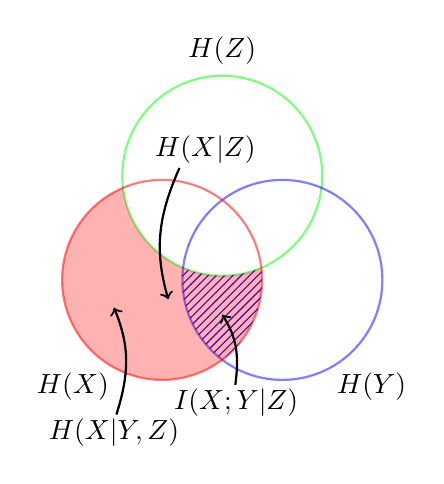
\begin{tikzpicture}
  \tikzstyle{set}=[
    circle,
    thick,
    draw opacity = .5,
    fill opacity = .3,
    text opacity = 1,
  ]
  \tikzstyle{arrow}=[{_[sep=-2px]}->, thick, opacity=1]
  \def\r{25px}
  \def\rc{36px}
  \def\circlez{(90:\r) circle (\rc)}
  \def\circley{(-30:\r) circle (\rc)}
  \def\circlex{(-150:\r) circle (\rc)}

  \draw[set, draw=green] \circlez node (z) {};
  \draw[set, draw=blue] \circley node (y) {};
  \draw[set, draw=red] \circlex node (x) {};

  \begin{scope}[even odd rule]
    \clip \circlex;
    \clip \circley;
    \fill[pattern=north east lines, pattern color=blue, fill opacity=.7] \circlez \circley;
  \end{scope}

  \begin{scope}[even odd rule]
    \clip \circlez \circlex;
    \fill[red, fill opacity=.3] \circlex;
  \end{scope}

  \node at ([shift={(90:45px)}]z) {$H(Z)$};
  \node at ([shift={(-50:50px)}]y) {$H(Y)$};
  \node at ([shift={(-130:50px)}]x) {$H(X)$};

  \node (hxyz) at (-120:78px) {$H(X|Y,Z)$};
  \draw[arrow] (hxyz.80) to [bend right=20] (-150:1.8*\r);

  \node (ixyz) at (-85:57px) {$I(X;Y|Z)$};
  \draw[arrow] (ixyz.90) to [bend right=20] (-90:\r);

  \node (hxz) at (100:35px) {$H(X|Z)$};
  \draw[arrow] (hxz.-140) to [bend right=20] (-135:1.1*\r);

\end{tikzpicture}
\end{document}
